\section{Reference banks, crossings and slow mixing}\label{sec:dynamics}

We have established all static inputs. It remains to use them along a path:
coverage selects references, fixed-scale locking controls incompatible
references, and narrow-annulus locking preserves constraints during
backwards searches. We first reduce Theorem~\ref{thm:main} to a sign
passage, then construct the required references, and finally bound the
probability of all resulting threshold constraints. As before,
$L=n^\kap$, $\rho=n^{-\kap}$, and constants may depend on the fixed
inverse temperature but not on $n$.

\subsection{Stationary paths and a sign-passage criterion}

Given $J$, start the discrete heat-bath chain $(x_k)_{k\ge0}$ at
$x_0\sim\pi^J$. Each step chooses a uniform site and resamples its spin
from the conditional Gibbs law. Stationarity gives marginal $\pi^J$
at every deterministic index. If $N$ is an independent rate-$n$ Poisson
process, $x_{N(t)}$ has conditional transition kernel $P_t^J$ from the
realized $x_0$. We work up to the deterministic index
\begin{equation}\label{eq:dyn-time-horizon}
 m=\lceil e^{2L}\rceil.
\end{equation}
Markov's inequality gives
\begin{equation}\label{eq:dyn-poisson-tail}
 \PP\{N(e^L)>m\}\leq \frac{ne^L}{m}\leq ne^{-L}=o(1).
\end{equation}
For every fixed configuration $v$, the overlap $R(v,x_k)$ changes by at
most $2/n$ at a single step.

A \emph{bank} is an ordered list of independent $\pi^J$ samples. Given
$J$, all raw bank entries are mutually independent and independent of
the complete path. Their sizes are deterministic functions of $n$.
A chosen reference may be reversed in sign at selection; that
orientation is thereafter fixed.

Suppose a first bank is used to select a reference $v_1$ satisfying
$R(v_1,x_0)\geq q_*$, with the choice and orientation depending only on
$J,x_0$ and this bank. Write $\mathcal S$ for successful selection, and
define its sign-passage event by
\[
 \mathcal A=\mathcal S\cap
 \{R(v_1,x_k)\leq0\text{ for some }0\leq k\leq m\}.
\]
Also write
\[
 \mathcal M=\left\{
 \norm{P_{e^L}^J(x_0,\cdot)-\pi^J}_{\TV}\leq\frac14\right\}.
\]
Spin-flip symmetry implies, for every oriented $v$,
\[
 \pi^J\{z:R(v,z)\leq0\}\geq\frac12.
\]
Condition on $J,x_0$ and successful first-bank selection. Since that
selection uses no future updates, the path and clock still have their
original conditional laws. On $\mathcal M$, total variation therefore
puts conditional probability at least $1/4$ on the opposite-sign
half-space at time $e^L$. Removing clock overruns gives
\begin{equation}\label{eq:dyn-tv-bridge}
 \PP(\mathcal A)\geq
 \frac14\PP(\mathcal M\cap\mathcal S)
 -\PP\{N(e^L)>m\}.
\end{equation}
Thus the remaining task is concrete: make the first reference available
with probability tending to one, and make its sign passage have
probability tending to zero.

Choose a fixed $b\in(0,1)$ no larger than the small-overlap cutoff in
Lemma~\ref{lem:fixed-locking} with large-overlap cutoff $q_*$. Next choose
$b'\in(0,b)$ no larger than that lemma's small-overlap cutoff with
large-overlap cutoff $b$. Fix $t_0>0$ so small that
\begin{equation}\label{eq:dyn-t0-choice}
 4t_0<\min\{q_*,b',b^2/2\}.
\end{equation}
We use the notation
\begin{equation}\label{eq:dyn-fixed-error}
 \eta_n=n^{-1/100}=\rho^{100}
\end{equation}
for the scale in fixed-scale locking.

\subsection{The case with a fixed forbidden overlap interval}

There are two possible scalar regimes. In the first,
$\Gamma(z)=z$ fails at some point of $(t_0/2,3t_0)$. Continuity then
supplies fixed constants
\[
 t_0/2<a_0<a_1<3t_0,\qquad d_0>0,
\]
such that $|q-\Gamma(q)|\geq d_0$ for all $q\in[a_0,a_1]$.
The pair gap~\eqref{static-eq:pair-pressure},
Lemma~\ref{lem:pressure-prob}, and the polynomial number of feasible pair
overlaps imply, for some $c>0$ and all sufficiently large $n$,
\begin{equation}\label{eq:dyn-fixed-forbidden}
 \EE\big[(\pi^J)^{\otimes2}
       \{(v,x):R(v,x)\in[a_0,a_1]\}\big]\leq e^{-cn}.
\end{equation}

Apply Proposition~\ref{prop:coverage} with $D_1=3$, let $D_3$ be its
constant, and take a single bank with
$K=\lceil\exp((D_3+1)L)\rceil$ entries. Select its first entry with
$|R(v,x_0)|\geq q_*$, oriented to give positive overlap. On the disorder
event of coverage for the whole configuration space, the Gibbs mass of
starting states whose qualifying neighborhood has mass below $e^{-D_3L}$
is at most $e^{-3L}$. For every other starting state, the independent bank
misses that neighborhood with probability at most $e^{-e^L}$. Hence
$\PP(\mathcal S)\to1$.

At a deterministic $k\le m$, the path point and a fixed signed bank
entry are independent Gibbs draws conditional on $J$. Sum
\eqref{eq:dyn-fixed-forbidden} over entries, signs and indices:
\[
 \PP\{R(\sigma v,x_k)\in[a_0,a_1]
     \text{ for some bank entry }v,\ \sigma\in\{-1,1\},\ k\leq m\}
 \leq 2K(m+1)e^{-cn}=o(1).
\]
For large $n$, a sequence beginning at overlap at least $q_*>a_1$ and
reaching nonpositive overlap, with jumps at most $2/n<a_1-a_0$, must visit
$[a_0,a_1]$. Therefore $\PP(\mathcal A)\to0$. Together with
\eqref{eq:dyn-tv-bridge}, this proves the theorem in this case.

This completes the forbidden-interval case. In the second regime we have
\begin{equation}\label{eq:dyn-identity-interval}
 \Gamma(z)=z\qquad(t_0/2<z<3t_0),
\end{equation}
and put
\begin{equation}\label{eq:dyn-local-scales}
 h=\rho^8,\qquad \varepsilon=\rho^{20}.
\end{equation}

\subsection{Thresholds and simultaneous bank properties}

Define the fixed integers and the number of levels by
\begin{equation}\label{eq:dyn-block-parameters}
 H_0=\lceil 2/b^2\rceil,\qquad B=H_0+2,\qquad
 p=B\left\lfloor\frac{t_0}{5B\rho}\right\rfloor.
\end{equation}
For large $n$, $p\ge B$. Divide the $p$ levels into consecutive blocks
of $B$ levels each. At the first level of every block after the first,
we \emph{reset} the selection cell to the whole space. Older retained
references are kept unless they meet the conflict rule specified below.
Independently of the disorder, banks and path, draw independent
thresholds $r_i$, uniform on
\begin{equation}\label{eq:dyn-threshold-intervals}
 I_i=[t_0+4(i-1)\rho,\ t_0+(4(i-1)+1)\rho].
\end{equation}
These intervals lie in $[t_0,2t_0]$, and
\begin{equation}\label{eq:dyn-threshold-separation}
 r_j-r_i\geq3\rho\qquad(i<j).
\end{equation}
Fubini's theorem gives
\[
 \EE\big[\mu([r_i-2h,r_i+2h])\big]\leq\frac{4h}{\rho}.
\]
Consequently Markov's inequality and a union bound show that the event
\begin{equation}\label{eq:dyn-threshold-good}
 \mathcal T=\{\mu([r_i-2h,r_i+2h])\leq\rho^4
                   \text{ for every }1\leq i\leq p\}
\end{equation}
satisfies
\begin{equation}\label{eq:dyn-threshold-good-prob}
 \PP(\mathcal T^c)\leq\frac{4ph}{\rho^5}=O(\rho^2).
\end{equation}
The Fubini calculation includes atoms; no regularity of the distribution
of the minimizing measure is imposed here.

There will be a bank $\mathcal B_j$ at every level. Its size must
compensate for the number of earlier reference tuples that can define
the selection cell. Using all preceding levels would give a recursion
of growing depth $p$; Proposition~\ref{prop:coverage} does not control
its constants uniformly in $n$. The reset confines this recursion to
$B$ fixed steps.
Bank sizes can then depend only on the position within a block, keeping
the total number of samples at $\exp(O(L))$. Older retained references
will still enter the crossing constraints below.

We require coverage for every possible earlier tuple in the current
block. For entries $u_i\in\mathcal B_i$ from those earlier levels, define
\begin{equation}\label{eq:dyn-cell}
 S=\{z:|R(u_i,z)|\leq3t_0
                    \text{ for every index in this tuple}\}.
\end{equation}
The empty tuple gives the whole space. We require
\begin{equation}\label{eq:dyn-bank-property}
 x_k\in S,\quad 0\leq k\leq m
 \quad\Longrightarrow\quad
 \text{some }w\in\mathcal B_j\cap S
          \text{ satisfies }|R(w,x_k)|\geq q_*.
\end{equation}
Absolute values make this property insensitive to orientations.

Choose the bank sizes recursively over the fixed positions
$s=1,\ldots,B$. Once the constants at smaller positions are fixed, set
\[
 C_s=\sum_{u<s}(D_{3,u}+2),\qquad D_{1,s}=C_s+5.
\]
Let $D_{3,s}$ be a constant supplied by
Proposition~\ref{prop:coverage} for $D_{1,s}$, and use
\[
 K_s=\lceil\exp((D_{3,s}+1)L)\rceil
\]
entries at position $s$. For large $n$, the number of earlier tuples in
the block is at most $\exp(C_sL)$. Only $B$ fixed applications of coverage
are needed, so their disorder events have an intersection $\mathcal D$
with $\PP(\mathcal D)\to1$.

Fix a level at position $s$, a realization $J\in\mathcal D$, and its
earlier bank lists. Each cell $S$ has a bad subset
\[
 B_S=\{x\in S:\pi^J\{z\in S:|R(z,x)|\geq q_*\}<e^{-D_{3,s}L}\}
\]
of Gibbs mass less than $e^{-D_{1,s}L}$. The path is independent of those
lists given $J$, and each deterministic-index marginal is $\pi^J$.
A union bound over tuples and deterministic indices therefore bounds the
probability that any $x_k$ lies in its cell's bad subset by
\[
 (m+1)e^{(C_s-D_{1,s})L}=O(e^{-3L}).
\]
After excluding these bad targets, condition also on the complete path.
The bank at the present level is still fresh. Its probability of missing
a qualifying neighborhood inside the cell is at most
\[
 (1-e^{-D_{3,s}L})^{K_s}\leq e^{-e^L}.
\]
Union over the same tuples and indices, and then over the $p=O(L)$
levels, shows that \eqref{eq:dyn-bank-property} holds simultaneously with
probability $1-o(1)$. The recursion has only $B$ steps, so the total number
of entries across all $p$ banks is $\exp(O(L))$.

We also impose simultaneous avoidance of the exceptional triples in
Lemma~\ref{lem:fixed-locking}, for the two cutoff pairs $(q_*,b)$ and
$(b,b')$, and in Lemma~\ref{lem:narrow-locking}. We do so for every
ordered triple of signed entries from distinct banks, and for every
ordered triple consisting of two signed entries from distinct banks and
one path point $x_k$, $0\leq k\leq m$. For each deterministic choice,
the conditional law given $J$ is $(\pi^J)^{\otimes3}$: bank independence,
stationarity at that deterministic index, and spin-flip symmetry suffice.
The sampled configurations themselves need not be different.

There are $\exp(O(L))$ such choices, including all orders and signs.
The exceptional probability for each is bounded by a constant times
$e^{-n^{9/10}}+e^{-n^{4/5}}$. A union bound thus makes all these locking
assertions simultaneous with probability $1-o(1)$. Let $\mathcal G$ be
the intersection of this event, the simultaneous bank property, and
$\mathcal T$. We have proved
\begin{equation}\label{eq:dyn-good-event-prob}
 \PP(\mathcal G^c)=o(1).
\end{equation}
We have made all these estimates simultaneously before choosing references
or crossing times. Later application at a backwards crossing therefore
uses this deterministic-index event, not an assertion of stationarity
at a random time.

\subsection{Backwards searches and deletion of conflicts}

Select $v_1$ from $\mathcal B_1$ as the first entry whose absolute overlap
with $x_0$ is at least $q_*$, and orient it positively. If it exists, let
$\tau_1$ be the first $k\leq m$ with $R(v_1,x_k)\leq r_1$. On success
initialize the ordered retained list as $A_1=\{1\}$.

At a subsequent level $j$, assuming all earlier levels have succeeded,
form the cell \eqref{eq:dyn-cell} using the selected references in earlier
positions of the current block. Choose as $v_j$ the first entry of
$\mathcal B_j$ lying in this cell and having absolute overlap at least
$q_*$ with $x_{\tau_{j-1}}$. Orient it so that
$R(v_j,x_{\tau_{j-1}})\geq q_*$. From $A_{j-1}$ delete the conflicts,
namely those indices $i$ with
\begin{equation}\label{eq:dyn-conflict}
 |R(v_i,v_j)|>b.
\end{equation}
The remaining old indices are called compatible. Search backwards from
$\tau_{j-1}$, stopping at the first point encountered with overlap at
most $r_j$ with $v_j$. Equivalently, if the set is nonempty, define
\begin{equation}\label{eq:dyn-backward-time}
 \tau_j=\max\{0\leq k\leq\tau_{j-1}:R(v_j,x_k)\leq r_j\}.
\end{equation}
Add $j$ to the compatible list to obtain $A_j$.

To use independence of each fresh threshold, define $v_j$ on failure
realizations as well. A missing candidate or missing crossing ends
the procedure. A candidate already selected before its crossing fails is
kept as that level's reference. At a level with no candidate, and at all
levels after an earlier failure, use the first entry of the corresponding
bank without sign reversal. These defaults serve the final conditional-probability calculation.
Selection and orientation of $v_j$ use only thresholds earlier than
$r_j$; its own threshold is used solely for the subsequent crossing. The first reference, when selected successfully, uses only
$J,x_0$ and $\mathcal B_1$ as required by
\eqref{eq:dyn-tv-bridge}.

We now work deterministically on $\mathcal G\cap\mathcal A$.
For all sufficiently large $n$, we will show that every level succeeds,
that reference $1$ survives, and that
\begin{align}
 |R(v_i,x_{\tau_j})-r_i|&\leq6j\varepsilon
                  &&(i\in A_j),\label{eq:dyn-induction-path}\\
 |R(v_i,v_\ell)-r_i|&\leq6j\varepsilon
                  &&(i,\ell\in A_j,\ i<\ell).
                  \label{eq:dyn-induction-references}
\end{align}
The induction also keeps the current block complete: after level $j$,
all references from that block's first level through $j$ remain on the
list. At the next reset, the preceding block is therefore intact.
Older blocks may already have gaps, but the complete preceding block
will prevent a new deletion from reaching them.
\begin{figure}[t]
\centering
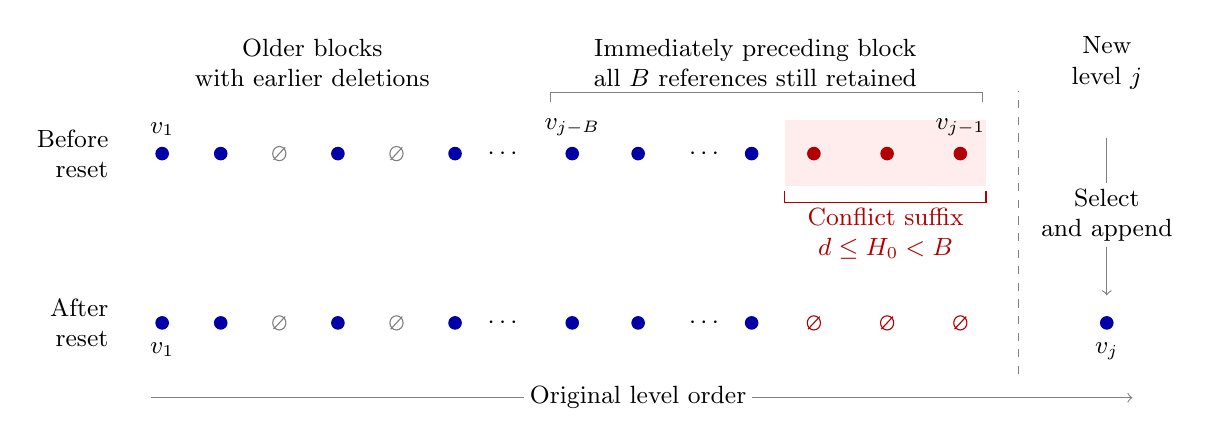
\begin{tikzpicture}[x=0.93cm,y=1cm,
  every node/.style={font=\small},
  kept/.style={circle,draw=blue!65!black,fill=blue!65!black,
               inner sep=0pt,minimum size=4.5pt},
  conflict/.style={circle,draw=red!70!black,fill=red!70!black,
                   inner sep=0pt,minimum size=4.5pt}]
  \node[align=center] at (3.35,3.45) {Older blocks\\with earlier deletions};
  \node[align=center] at (9.4,3.45)
      {Immediately preceding block\\all $B$ references still retained};
  \node[align=center] at (14.2,3.45) {New\\level $j$};
  \draw[gray] (6.6,2.96)--(6.6,3.08)--(12.5,3.08)--(12.5,2.96);
  \draw[gray,dashed] (13.0,-0.50)--(13.0,3.10);
  \node[anchor=east,align=right] at (0.7,2.30) {Before\\reset};
  \node[anchor=east,align=right] at (0.7,0.15) {After\\reset};

  \foreach \y in {2.30,0.15} {
    \foreach \x in {1.3,2.1,3.7,5.3}
      \node[kept] at (\x,\y) {};
    \foreach \x in {2.9,4.5} {
      \draw[gray] (\x,\y) circle[radius=0.09];
      \draw[gray] (\x-0.08,\y-0.08)--(\x+0.08,\y+0.08);
    }
    \node at (5.95,\y) {$\cdots$};
  }
  \node[above] at (1.3,2.40) {$v_1$};
  \node[below] at (1.3,0.02) {$v_1$};

  \fill[red!7] (9.80,1.89) rectangle (12.55,2.73);
  \foreach \x in {6.9,7.8}
    \node[kept] at (\x,2.30) {};
  \node at (8.7,2.30) {$\cdots$};
  \node[kept] at (9.35,2.30) {};
  \foreach \x in {10.2,11.2,12.2}
    \node[conflict] at (\x,2.30) {};
  \node[above] at (6.9,2.40) {$v_{j-B}$};
  \node[above] at (12.2,2.40) {$v_{j-1}$};
  \draw[red!70!black] (9.80,1.83)--(9.80,1.68)--(12.55,1.68)--(12.55,1.83);
  \node[text=red!70!black,align=center] at (11.18,1.28)
      {Conflict suffix\\$d\le H_0<B$};

  \foreach \x in {6.9,7.8,9.35}
    \node[kept] at (\x,0.15) {};
  \node at (8.7,0.15) {$\cdots$};
  \foreach \x in {10.2,11.2,12.2} {
    \draw[red!70!black] (\x,0.15) circle[radius=0.09];
    \draw[red!70!black] (\x-0.08,0.07)--(\x+0.08,0.23);
  }
  \node[kept] at (14.2,0.15) {};
  \node[below] at (14.2,0.02) {$v_j$};
  \draw[->,gray] (14.2,2.50)--(14.2,0.50);
  \node[align=center,fill=white,inner sep=2pt] at (14.2,1.52)
      {Select\\and append};

  \draw[->,gray] (1.15,-0.80)--(14.55,-0.80);
  \node[fill=white,inner sep=2pt] at (7.8,-0.80) {Original level order};
\end{tikzpicture}
\caption{Why a reset preserves the first reference. The dots are schematic
slots in the original level order; omitted entries are indicated by
ellipsis, and crossed gray slots represent deletions at earlier resets.
Immediately before a reset at level $j$, the preceding block
$\{j-B,\ldots,j-1\}$ is complete. Conflicts form a suffix of the retained
list of length $d\le H_0<B$, illustrated in red. The suffix therefore
misses both the first reference of that complete block and all older
retained references. Thus $v_1$ survives at the first reset, when it
belongs to the preceding block, and at every later reset, as drawn.
The new reference $v_j$ is then appended.
Older blocks may contain holes and need not be complete. The diagram
illustrates a nonempty conflict suffix; the proof also permits $d=0$.}
\label{fig:protected-block}
\end{figure}


Deletions occur only at the first level of a new block, and at most $H_0$
indices, forming a suffix of the old list, are deleted at each such level.

At level $1$, coverage of the whole space supplies the reference.
Sign passage forces the first crossing, where the one-step overlap
bound puts the value in $[r_1-2/n,r_1]$. This starts the induction. In the following induction we
use the scale relations
\begin{equation}\label{eq:dyn-scale-relations}
 \frac1n\ll\eta_n=\rho^{100}\ll\varepsilon=\rho^{20},\qquad
 p\varepsilon=O(\rho^{19})\ll h=\rho^8\ll\rho.
\end{equation}

Suppose the assertions hold through level $j-1$. All earlier references
in the current block are still retained, since there have been no
deletions within that block after its first level. Their overlaps with
$x_{\tau_{j-1}}$ have absolute value at most
$2t_0+6p\varepsilon<3t_0$. Thus this target belongs to the required cell,
and the new selection $w=v_j$ exists by
\eqref{eq:dyn-bank-property}.

For each compatible old index $i$, the two small overlaps in the triple
$(v_i,w,x_{\tau_{j-1}})$ have absolute value at most $b$, whereas
$R(w,x_{\tau_{j-1}})\geq q_*$. Fixed-scale locking gives
\begin{equation}\label{eq:dyn-target-transfer}
 |R(v_i,w)-R(v_i,x_{\tau_{j-1}})|\leq2\eta_n.
\end{equation}
In particular,
\begin{equation}\label{eq:dyn-reference-transfer}
 |R(v_i,w)-r_i|\leq6(j-1)\varepsilon+2\eta_n
 \qquad(i\text{ compatible}).
\end{equation}

\par\medskip\noindent\textbf{Conflicts occupy a bounded final segment.}\enspace
A conflicting old index $i$ cannot precede a compatible old index $\ell$. Indeed, by
\eqref{eq:dyn-induction-references} and
\eqref{eq:dyn-reference-transfer}, the magnitudes of
$R(v_\ell,v_i)$ and $R(v_\ell,w)$ are within
$6(j-1)\varepsilon$ and $6(j-1)\varepsilon+2\eta_n$ of $r_i$ and
$r_\ell$, respectively.
Both magnitudes are less than $b'$, by
\eqref{eq:dyn-t0-choice}. Their difference in magnitude is at least
\[
 3\rho-12p\varepsilon-2\eta_n>2\eta_n.
\]
On the other hand $|R(v_i,w)|>b$. Reverse one of this pair if necessary
to make their mutual overlap positive. The signed difference of the two
small overlaps has absolute value at least their difference in magnitude.
This contradicts fixed-scale locking with cutoff pair $(b,b')$, which
holds for all signs on $\mathcal G$. The conflicts consequently form a
suffix of the old retained list.

The number of conflicts is bounded by $H_0$. Indeed, the induction
bounds all absolute overlaps between retained old references by
$2t_0+6p\varepsilon<3t_0$. If $d\geq1$ of them conflict with $w$,
normalize them to unit vectors and reverse each sign to give inner
product greater than $b$ with $w/\sqrt n$. Denote these vectors by
$u_1,\ldots,u_d$. Then
\[
 d^2b^2<\left\langle\sum_{a=1}^d u_a,\frac{w}{\sqrt n}\right\rangle^2
 \leq\norm{\sum_{a=1}^d u_a}^2
 \leq d+3t_0d(d-1).
\]
Since $3t_0<b^2/2$, this implies
\[
 d<\frac{1-3t_0}{b^2-3t_0}<\frac{2}{b^2}\leq H_0.
\]
In particular $d\leq H_0$.

If $j$ is not the first level of its block, the most recent old index
$j-1$ is compatible: the cell condition gives
$|R(v_{j-1},w)|\leq3t_0<b$. A suffix of conflicts is therefore empty.
At the first level of a new block, the additional invariant says that
all $B$ entries selected in the preceding block are still present. Removing at most $H_0<B$ final indices
cannot reach any older block, or the first index of the preceding block.
In particular index $1$ survives, including at the first reset. Adding the new index starts the current block as a retained singleton;
at a nonreset it extends the complete current block because there is no
deletion. This establishes the additional invariant and the deletion
claims before proving that the new crossing exists.

\par\medskip\noindent\textbf{The backwards search preserves old constraints.}\enspace
Follow the search for $\tau_j$, including the crossing step when there
is one. The new reference satisfies throughout this search
\begin{equation}\label{eq:dyn-search-large-overlap}
 R(w,x_k)\geq r_j-2/n.
\end{equation}
If there is no crossing, this follows with the stronger strict bound
$R(w,x_k)>r_j$ at every index down to zero. If there is a crossing, all
indices strictly after it have overlap greater than $r_j$, and the jump
bound gives \eqref{eq:dyn-search-large-overlap} at the crossing itself.

For each compatible old reference $v_i$,
\eqref{eq:dyn-reference-transfer} places the fixed value $R(v_i,w)$
near $r_i$. The larger threshold $r_j$ separates the new overlap from
that old level throughout the search. We will use narrow-annulus
locking to prove
\begin{equation}\label{eq:dyn-search-locking}
 |R(v_i,x_k)-R(v_i,w)|<2\varepsilon
\end{equation}
on this entire searched portion. Equation~\eqref{eq:dyn-target-transfer} proves the claim at the target.
At a first violation while moving backwards, the one-step bound puts
the left side in $[2\varepsilon,2\varepsilon+2/n]$. For this triple
use the parameters of Lemma~\ref{lem:narrow-locking}:
\[
 r=\frac{R(v_i,x_k)+R(v_i,w)}2,\qquad
 \delta=\frac{R(v_i,x_k)-R(v_i,w)}2,\qquad q=R(w,x_k).
\]
Then
\[
 \varepsilon\leq|\delta|\leq\varepsilon+1/n\leq2\varepsilon,
 \qquad
 |r-r_i|\leq6(j-1)\varepsilon+2\eta_n+\varepsilon+1/n<h.
\]
It follows that $t_0/2<r<3t_0$ and
$[r-h,r+h]\subseteq[r_i-2h,r_i+2h]$. Thus $\mathcal T$ gives the
required bound $\mu([r-h,r+h])\leq\rho^4$. Also, by
\eqref{eq:dyn-threshold-separation},
\eqref{eq:dyn-search-large-overlap}, and
\eqref{eq:dyn-scale-relations},
\[
 q-r\geq3\rho-6(j-1)\varepsilon-2\eta_n-\varepsilon-3/n
       \geq\rho.
\]
All conditions of the forbidden narrow-annulus event hold, contradicting
its simultaneous avoidance on $\mathcal G$. This proves
\eqref{eq:dyn-search-locking}.

The crossing must exist. Otherwise the search reaches index zero, and
\eqref{eq:dyn-reference-transfer}--\eqref{eq:dyn-search-locking}
apply there to the surviving compatible reference $1$. They would give
\[
 R(v_1,x_0)<r_1+6(j-1)\varepsilon+2\eta_n+2\varepsilon<q_*,
\]
contradicting the first selection. Hence the crossing exists. Its new
reference overlap belongs to $[r_j-2/n,r_j]$. For each retained old
reference, the error at the new crossing is at most
$6(j-1)\varepsilon+2\eta_n+2\varepsilon\leq6j\varepsilon$.
The old-new reference errors satisfy the same claimed bound by
\eqref{eq:dyn-reference-transfer}, and old-old reference errors are
unchanged. This proves
\eqref{eq:dyn-induction-path}--\eqref{eq:dyn-induction-references} and
completes the induction.

There are at most $p/B$ reset occasions, so the final list has size at least
\begin{equation}\label{eq:dyn-retained-count}
 |A_p|\geq p-H_0p/B\geq p/B.
\end{equation}
Consequently $\mathcal G\cap\mathcal A$ implies that, for some
index $k$ in $\{0,\ldots,m\}$ and some subset of $p/B$
indices, the inequalities
\begin{equation}\label{eq:dyn-small-target-windows}
 |R(v_i,x_k)-r_i|\leq6p\varepsilon
\end{equation}
hold simultaneously. We have reduced sign passage to this existence event. The probability
bound that follows will not condition on $\mathcal G$ or on the
random retained list.

\subsection{Predictable thresholds and completion of the proof}

Let $\mathcal F_0$ be generated by $J$, all raw bank lists, and the path
$(x_0,\ldots,x_m)$, and set
\[
 \mathcal F_i=\sigma(\mathcal F_0,r_1,\ldots,r_i),
 \qquad 1\leq i\leq p.
\]
Every $r_i$ is uniform on $I_i$ and independent of $\mathcal F_{i-1}$.
The failure conventions ensure that each oriented $v_i$ is
$\mathcal F_{i-1}$-measurable. Here is the complete induction. At level $1$ its
selection does not use any threshold. Inductively, whether a prior level
failed, the previously selected references, and the preceding crossing
time are all determined by earlier thresholds. Selection at level $i$
uses only that information and the bank and path data in $\mathcal F_0$.
The subsequent crossing may use $r_i$, but never changes that selected
reference. A default caused by an earlier failure likewise depends only
on earlier thresholds. This proves the claim, including on failure
events.

For each deterministic $k\leq m$, let
\[
 E_i(k)=\{|R(v_i,x_k)-r_i|\leq6p\varepsilon\},\qquad
 \gamma_n=\frac{12p\varepsilon}{\rho}.
\]
The interval defining $E_i(k)$ has length at most $12p\varepsilon$,
while $I_i$ has length $\rho$. Thus, for all sufficiently large $n$,
\begin{equation}\label{eq:dyn-conditional-window}
 \PP(E_i(k)\mid\mathcal F_{i-1})\leq\gamma_n<1.
\end{equation}
For a deterministic subset $\{i_1<\cdots<i_s\}$, the earlier events
$E_{i_1}(k),\ldots,E_{i_{s-1}}(k)$ are
$\mathcal F_{i_s-1}$-measurable. Conditioning first at the largest
selected index and using \eqref{eq:dyn-conditional-window} yields
\[
 \PP\left(\bigcap_{a=1}^s E_{i_a}(k)\right)
 \leq\gamma_n\,
 \PP\left(\bigcap_{a=1}^{s-1}E_{i_a}(k)\right)
 \leq\gamma_n^s.
\]
The elimination order is essential: the latest selected threshold is
integrated out first. Later centers may depend on earlier thresholds,
but the displayed conditioning remains valid. Neither the random
retained subset nor the good event has been conditioned on.

Taking $s=p/B$, then taking a union over all deterministic subsets and all
deterministic indices $k$, proves
\begin{equation}\label{eq:dyn-threshold-union}
 \PP\{\text{\eqref{eq:dyn-small-target-windows} holds for some }k
                  \text{ and some subset of size }p/B\}
 \leq(m+1)2^p\left(\frac{12p\varepsilon}{\rho}\right)^{p/B}
 =o(1).
\end{equation}
Indeed $p=(t_0/5)L+O(1)$, $\rho=L^{-1}$, and
$12p\varepsilon/\rho=O(\rho^{18})$. The logarithm of the right-hand
side is therefore bounded above by
\[
 2L+O(p)-\frac{18p}{B}\log(1/\rho)
       =-\Omega(L\log L).
\]

The deterministic induction and \eqref{eq:dyn-good-event-prob} now imply
\[
 \PP(\mathcal A)
 \leq\PP(\mathcal G^c)
       +\PP(\mathcal G\cap\mathcal A)=o(1).
\]
The first selection succeeds on the simultaneous bank event at level $1$,
so $\PP(\mathcal S^c)=o(1)$ as well. Finally,
\eqref{eq:dyn-tv-bridge} and \eqref{eq:dyn-poisson-tail} give
\[
 \PP(\mathcal M)
 \leq\PP(\mathcal S^c)+4\PP(\mathcal A)
       +4\PP\{N(e^L)>m\}=o(1).
\]
This proves Theorem~\ref{thm:main} also under
\eqref{eq:dyn-identity-interval}, and the two cases exhaust the
possibilities.

Finally take $T_n=\lfloor e^L\rfloor$ discrete update attempts.
This deterministic index lies below $m$ for large $n$. If its transition
law is within $1/4$ of equilibrium, the opposite-sign half-space has
conditional probability at least $1/4$ at that index. Thus the same
sign-passage inequality holds with no clock-overrun term. All bank,
locking and threshold estimates already concern the discrete path,
so they prove the second assertion of Theorem~\ref{thm:main} at exactly
$\lfloor e^L\rfloor$ attempts.
